% Descripcion
% Sergio Cuellar
% 24 Enero 12
% Reorganización del informe

\chapter{Descripción}
\label{chap:descripcion}

El área de Desarrollo de Sistemas de Restaurantes está conformado por cuatro personas encargadas de proveer varios servicios de apoyo a alrededor de 340 restaurantes propios de la franquicia de PRB, así como alrededor de 150 restaurantes de otros franquiciatarios. Los requerimientos de desarrollos nuevos son proporcionados generalmente por el área de Operaciones cuando éstos tienen que ver la operación misma del restaurante, o bien, por la misma área cuando se deben realizar actualizaciones, corrección de bugs, etc., al sistema.

\section{Objetivos}
\label{sec:objetivos}

Entre los servicios proporcionados por el área de Desarrollo de Sistemas de Restaurantes se encuentran:

\begin{itemize}
 \item Desarrollo y mantenimiento de reportes solicitados por el área de Operaciones.
 \item Mantenimiento al punto de venta (programación de mejoras, nuevas funcionalidades, corrección de bugs).
 \item Programación de herramientas que coadyuven a la eficaz operación del restaurante.
 \item Desarrollo de aplicaciones que contribuyan a disminuir el costo de operación.
 \item Investigación de nueva infraestructura de sistemas en el restaurante (impresoras, tarjetas de vídeo, terminales, etc.)
\end{itemize}

\section{Descripción del Sistema en restaurantes}
\label{sec:descripcion}

Cada uno de los restaurantes cuenta con una computadora, en la cual se efectúan diversos procesos como son:

\begin{itemize}
 \item Registro y procesamiento de la venta.
 \item Generación de reportes.
 \item Manejo de periféricos como impresora de tickets, impresora del gerente, cajas registradoras, terminales, etc.
 \item Actividades gerenciales (correo electrónico, consultas web de la intranet, uso de procesador de textos, hoja de cálculo, etc).
\end{itemize}

\subsection{Software Libre}
\label{subsec:software_libre}

Una de las características principales del sistema en restaurantes, es que casi en su totalidad, a excepción del punto de venta que fue desarrollado por la compañía, es software libre.

El software libre es software que puede ser usado, estudiado y modificado sin restricción y el cual puede ser copiado y redistribuido en su forma modificada u original, ya sea sin restricciones o con mínimas restricciones que aseguren que los siguientes usuarios del software puedan seguir haciendo estas actividades. El software libre es generalmente disponible sin cargo alguno pero puede tener algunas cuotas, por ejemplo para ser distribuido en forma de CDs u otras formas.

En la práctica, para que un software sea distribuido como software libre, el código fuente de éste debe estar disponible para el usuario, así como también indicarle en una nota que se le conceden los derechos arriba mencionados. Esta nota puede ser, ya sea, una licencia de software libre o indicando que el código fuente está disponible al dominio público.

Las ventajas del software libre son:

\begin{itemize}
 \item Bajo costo, lo que implica el ahorro en pago de licencias.
 \item Es posible adaptar el software a las necesidades que tenga cada usuario, teniendo como resultado un software personalizado.
 \item Al ser público el código fuente, permite que programadores hagan correcciones a errores y mejoren el software de manera rápida.
 \item De acuerdo a los dos últimos puntos, el software libre no depende de una única empresa u organización, lo que evita que se impongan condiciones en su uso, como ocurre con el software privado.
 \item La innovación tecnológica que surge gracias a que cada usuario puede hacer aportaciones a la mejora del software.
\end{itemize}

El sistema de software de los restaurantes se compone principalmente de:

\begin{itemize}
 \item Sistema Operativo GNU/Linux kernel 2.6, basado en Knoppix con escritorio Xfce.
 \item Apache Tomcat
 \item Servidor HTTP Apache
 \item PostgreSQL
 \item Mozilla Firefox
 \item Mozilla Thunderbird
 \item OpenOffice.org
 \item Herramientas GNU (bash, ksh, awk, perl, etc.)
 \item Sistema punto de venta SUS/FMS (propietario, desarrollado por la misma compañía.
\end{itemize}

\subsection{GNU/Linux}
\label{sec:linux}

GNU/Linux se refiere al sistema operativo que utiliza el kernel Linux y las herramientas GNU. El kernel Linux puede ser instalado en una gran variedad de hardware, desde teléfonos móviles, computadoras tipo tableta, consolas de videojuegos, hasta mainframes y supercomputadoras. El kernel de Linux fue iniciado en 1991 por el finlandés Linus Torvalds. Las herramientas del sistema y librerías conocidas como GNU, fueron en un principio desarrolladas por Richard Stallman en 1983.

Algunas características del kernel de Linux son:

\begin{itemize}
 \item Es multitareas, permite ejecutar diferentes programas al mismo tiempo.
 \item Es multiusuario, distintos usuarios pueden estar conectados a la misma computadora al mismo tiempo.
 \item Es multiplataforma, puede ser instalado en distintos tipo de arquitectura de procesadores.
 \item Es multihilo, Linux tiene soporte en kernel nativo para el control de múltiples hilos independientes.
 \item Tiene soporte a una gran cantidad de sistemas de archivos (ext2, ext3, ext4, ReiserFS, XFS, JFS, FAT32, etc.).
\end{itemize}


\subsection{Apache Tomcat}
\label{sec:tomcat}

Apache Tomcat o simplemente Tomcat es un contenedor de servlets desarrollado por la Apache Software Foundation. Tomcat implementa las especificaciones de Java Servlet y JavaServer Pages (JSP) de Sun Microsystems (ahora Oracle).

Un servlet es un tipo de clase de Java que es usada para extender las capacidades de un servidor que contienen aplicaciones que son accedidas mediante un modelo de programación petición-respuesta. Si bien, un servlet puede responder cualquier tipo de petición, son comúnmente usados en aplicaciones contenidas en un servidor web.

Los JavaServer Pages, mejor conocidos como JSPs es una tecnología de Java que ayuda a los desarrolladores de software a generar páginas web de manera dinámica basadas en HTML, XML o algún otro tipo de documento.

\subsection{Servidor HTTP Apache}
\label{sec:apache}

El servidor HTTP Apache, o mejor conocido únicamente como Apache, es un servidor web que implementa el protocolo HTTP/1.1. Una de las mayores ventajas de Apache es que puede ser mejorado con la ayuda de módulos compilados que extienden la funcionalidad del servidor. Hay módulos que permiten la interacción con distintos lenguajes de programación como Perl, Pyhton, PHP, etc. Existen módulos de autenticación para aumentar la seguridad del servidor, como mod\_auth, mod\_access, etc. Una de las características más importantes de Apache es el manejo de host virtuales, lo que permite que un servidor Apache maneje diferentes sitios web.

Tomcat y Apache pueden ser conectados a través del conector mod\_jk. Eso es de gran ayuda, por ejemplo, cuando se tienen páginas programadas en PHP y en JSP, y se quiere tener un único puerto de acceso a la página principal. Con mod\_jk, Apache recibe todas las peticiones y les da respuesta únicamente las de tipo PHP y HTML, y redirige a Tomcat las que tienen que ver con JSPs. Esta implementación la realicé en PRB para evitar el uso del puerto 80 para reportes en PHP y el 8080 para reportes programados en JSP. Se unificó el URL que es ingresado en los restaurantes.

\subsection{PostgreSQL}
\label{sec:postgresql}

PostgreSQL, o simplemente Postgres, es un sistema de gestión de base de datos relacional orientada a objetos (ORDBMS\footnote{object-relational database management system}). Algunas de sus características son:

\begin{itemize}
 \item Uso de lenguajes procedurales o mejor conocidos como \textit{store procedures}, permiten que bloques de código sean ejecutados por el servidor de base de datos y pueden ser escritos en lenguajes de programación distintos a SQL y C; y sirven para crear funciones definidas por el usuario (subrutinas, triggers, etc.). Pueden ser programados en Perl, Python, pgSQL, Tcl, principalmente.
 \item Uso de índices, triggers, transacciones anidadas, vistas.
 \item Numerosos tipos de datos y posibilidad de definir nuevos.
 \item Posee interfases de programación de aplicaciones (API\footnote{Application Programming Interface} en varios lenguajes como C, C++, Java, Perl, Ruby, PHP, entre otros.
 \item Es 100\% ACID\footnote{\textit{Atomicity, Consistency, Isolation, Durability}. En base de datos se denomina ACID a un conjunto de características necesarias para que una serie de instrucciones puedan ser consideradas como una transacción.}
\end{itemize}

\subsection{Mozilla Firefox}
\label{sec:firefox}

Mozilla Firefox es un navegador web disponible para varios sistemas operativos como Microsoft Windows, GNU/Linux, Mac OS X, FreeBSD y muchos otros. Para la visualización de páginas web, Firefox utiliza a Gecko, que es un motor de renderizado, que implementa la mayoría de los estándares web. Algunas de las características de Firefox son:

\begin{itemize}
 \item Navegación por pestañas.
 \item Corrector ortográfico.
 \item Navegación privada.
 \item Soporte de complementes (plug-ins) desarrollados por terceros para incrementar la funcionalidad del navegador.
 \item Administrador de descargas.
\end{itemize}

\subsection{Mozilla Thunderbird}
\label{sec:thunderbird}

Mozilla Thunderbird es un cliente de correo electrónico y noticias. Puede manejar múltiples cuentas de correo electrónico y noticias. Características como son la búsqueda rápida, filtrado de mensajes, agrupamiento de mensajes y etiquetas ayudan a manejar y encontrar mensajes de una manera fácil. Thunderbird incorpora un filtro de spam tipo Bayesiano para la clasificación de correo no deseado. Al igual que Firefox, a Thunderbird le pueden ser instalados complementos o extensiones que amplían la funcionalidad de éste. Soporta POP e IMAP, así como LDAP para el manejo de la libreta de direcciones. Está disponible para varios sistemas operativos como Microsoft Windows, GNU/Linux, Mac OS X, Opensolaris, etc.

\subsection{OpenOffice.org}
\label{sec:openoffice}

OpenOffice.org es una suite de aplicaciones cuyos componentes principales son procesador de palabras, hoja de cálculo, presentaciones, gráficas y base de datos. Está disponible para distintos sistemas operativos. El formato nativo de OpenOffice.org es el estándar ISO/IEC OpenDocument (ODF), pero también soporta la lectura y en la mayoría, la escritura de formatos propietarios como los de WordPerfect, StarOffice, MS Works, Rich Text format, los formatos de Microsoft Office, entre otros.

Posee diccionarios ortográficos en varios idiomas. Puede usar extensiones para agregar funciones adicionales. Las aplicaciones incluidas con OpenOffice.org son:

\begin{itemize}
 \item OpenOffice.org Writer es el procesador de textos. Una de las características de Writer es que permite exportar documentos a PDF y HTML sin software adicional.
 \item OpenOffice.org Calc es una hoja de cálculo similar a Microsoft Excel, pero con más características.
 \item OpenOffice.org Impress es el programa usado para realizar presentaciones similares a Microsoft PowerPoint. Puede exportar presentaciones al formato SWF, permitiendo visualizar la presentación en cualquier computadora que cuente con un reproductor Flash.
 \item OpenOffice.org Base es un programa similar a Microsoft Access, el cual permite la creación y manejo de base de datos, elaboración de formularios y reportes.
 \item OpenOffice.org Draw es un editor de gráficos vectoriales y herramienta para elaborar diagramas, similar a Microsoft Visio.
 \item OpenOffice.org Math es una aplicación diseñada para la creación y edición de fórmulas matemáticas. Las fórmulas pueden ser incorporadas a otros documentos de OpenOffice.org, como en un documento de Writer o bien exportar la fórmula a otro formato de archivo como PDF.
\end{itemize}

\subsection{Sistema Punto de Venta SUS}
\label{sec:sus}

El sistema punto de venta utilizado tanto en PH como en KFC se llama SUS, el cual fue desarrollado por el área de desarrollo de Yum Restaurants de Estados Unidos. Nosotros contamos con el código fuente, con el cual podemos corregir errores, añadir funcionalidades o mejorar las ya existentes. El punto de venta no es software libre.

SUS es capaz de realizar toma de ordenes, el despacho de estas ordenes, retiros, funciones de control y actividades administrativas propias de un restaurante.

El sistema SUS divide las actividades realizadas en el restaurante en las siguientes áreas:

\begin{itemize}
 \item Toma de ordenes.
 \item Control de efectivo.
 \item Funciones administrativas.
 \item Inventarios.
 \item Control de asistencia.
 \item Mantenimiento de tablas del sistema.
 \item Reportes.
\end{itemize}

Estas áreas corresponden también a las áreas en las que se les puede asignar responsabilidad al equipo del restaurante. Cada nivel de responsabilidad, junto con el asociado cuenta con un nombre de usuario y contraseña. Esto permite la asignación de responsabilidades, limitando el acceso a partes del sistema con información importante de los clientes y del restaurante.

\subsubsection{Toma de ordenes}
\label{sec:sus_toma_ordenes}

Esta función se utiliza principalmente en Pizza Hut, y en KFC en los restaurantes con servicio de entrega a domicilio, en donde es de suma importancia, que cada producto sea rápida y fácilmente ordenado para toda ocasión, de esta manera se agiliza enormemente el proceso de toma de ordenes.

\subsubsection{Control de Efectivo y despacho}
\label{sec:sus_control_efectivo}

Las funciones de esta parte del punto de venta permiten realizar retiros de dinero de manera eficiente 

\subsection{e-Reports}
\label{sec:ereports}

\textit{e-Reports} es una herramienta desarrollada para consultar reportes via web, mediante Firefox, utilizando el servidor Tomcat junto con la base de datos de PostgreSQL. Cada restaurante cuenta con este reporteador para realizar distintas actividades, como son, la consulta de su inventario, la captura de gastos semivariables, conocer el número de transacciones mediante gráficas, etc. Es una de las herramientas más usadas en los restaurantes, junto con el punto de venta, debido a la gran cantidad de información que se puede consultar. Al ser una herramienta web, ésta puede ser consultada desde cualquier computadora que pertenezca a la VPN y conozca la clave para ingresar.

Los reportes son programados en JSP, JavaScript y en algunos casos se hace uso de scripts externos desarrollados en Perl y Bash principalmente. Además, se cuenta con una API desarrollada especialmente para e-Reports, en la cual ya existen métodos para la conexión a base de datos, la creación de tablas dinámicas, conversión de resultados de consulta de base de datos a arreglos de JavaScript, etc. El framework de JavaScript utilzado es BlueShoes\footnote{http://www.blueshoes.org/en/javascript/}.

\begin{figure}[htb]
 \begin{center}
  \includegraphics[scale=0.5]{ereports_1.png}
 \end{center}
 \caption{Página principal de e-Reports}
 \label{fig:ereports}
\end{figure}

\subsection{Reporteador}
\label{sec:reporteador}

Existe otra herramienta para consultar reportes via web llamado \textit{Reporteador}, el cual, a diferencia de \textit{e-Reports}, es usado en mayor parte de los reportes que posee, para desplegar información relacionada directamente con reportes generados por el mismo punto de venta. El despliegue de estos reportes es programado en HTML, PHP y algunos CGI's\footnote{Common Gateway Interface} en Python. Se puede decir que \textit{e-Reports} y el \textit{Reporteador} se complementan, pero en un futuro, el plan es migrar todos los reportes de este último, para concentrar todo en \textit{e-Reports}.

El \textit{Reporteador} posee una clasificación de reportes, la cual está conformada por:

\begin{itemize}
 \item Ingresos y gastos: Ventas Diarias, Ventas por Hora, Operaciones Diarias, Cancelaciones Diarias, Auditoría de Cajero y Ventas pollo por hora (para KFC).
 \item Inventarios: Inventario de críticos, usos ideales, Ordenes de compra, Recepciones.
 \item Mano de Obra: Modelo de Labor.
 \item Estadísticas: Pronóstico y Ensamble, Historial de Pedidos, Mix Diario por Productos, Mix por Cajero, Estadística Diaria.
 \item Home Service: Auditoría de Repartidor, Reporte de Vendedores, Mapa por calles, Mapa de Calles, etc.
 \item Planeación: Ya no cuenta con algún reporte.
 \item Auditoría: Notas de consumo, Retiros Parciales, Depósitos de Dólares.
 \item Utilerías: Ya no cuenta con algún reporte.
\end{itemize}

El \textit{Reporteador} y \textit{e-Reports} conviven en la misma dirección y mismo puerto gracias al mod\_jk, descrito en \ref{sec:apache}

\begin{figure}[htb]
 \begin{center}
  \includegraphics[scale=0.5]{reporteador_1.png}
 \end{center}
 \caption{Reporteador}
 \label{fig:reporteador}
\end{figure}

A continuación se muestran un diagrama que representa a muy grandes rasgos el sistema en Pizza Hut:

\begin{figure}[htb]
 \begin{center}
  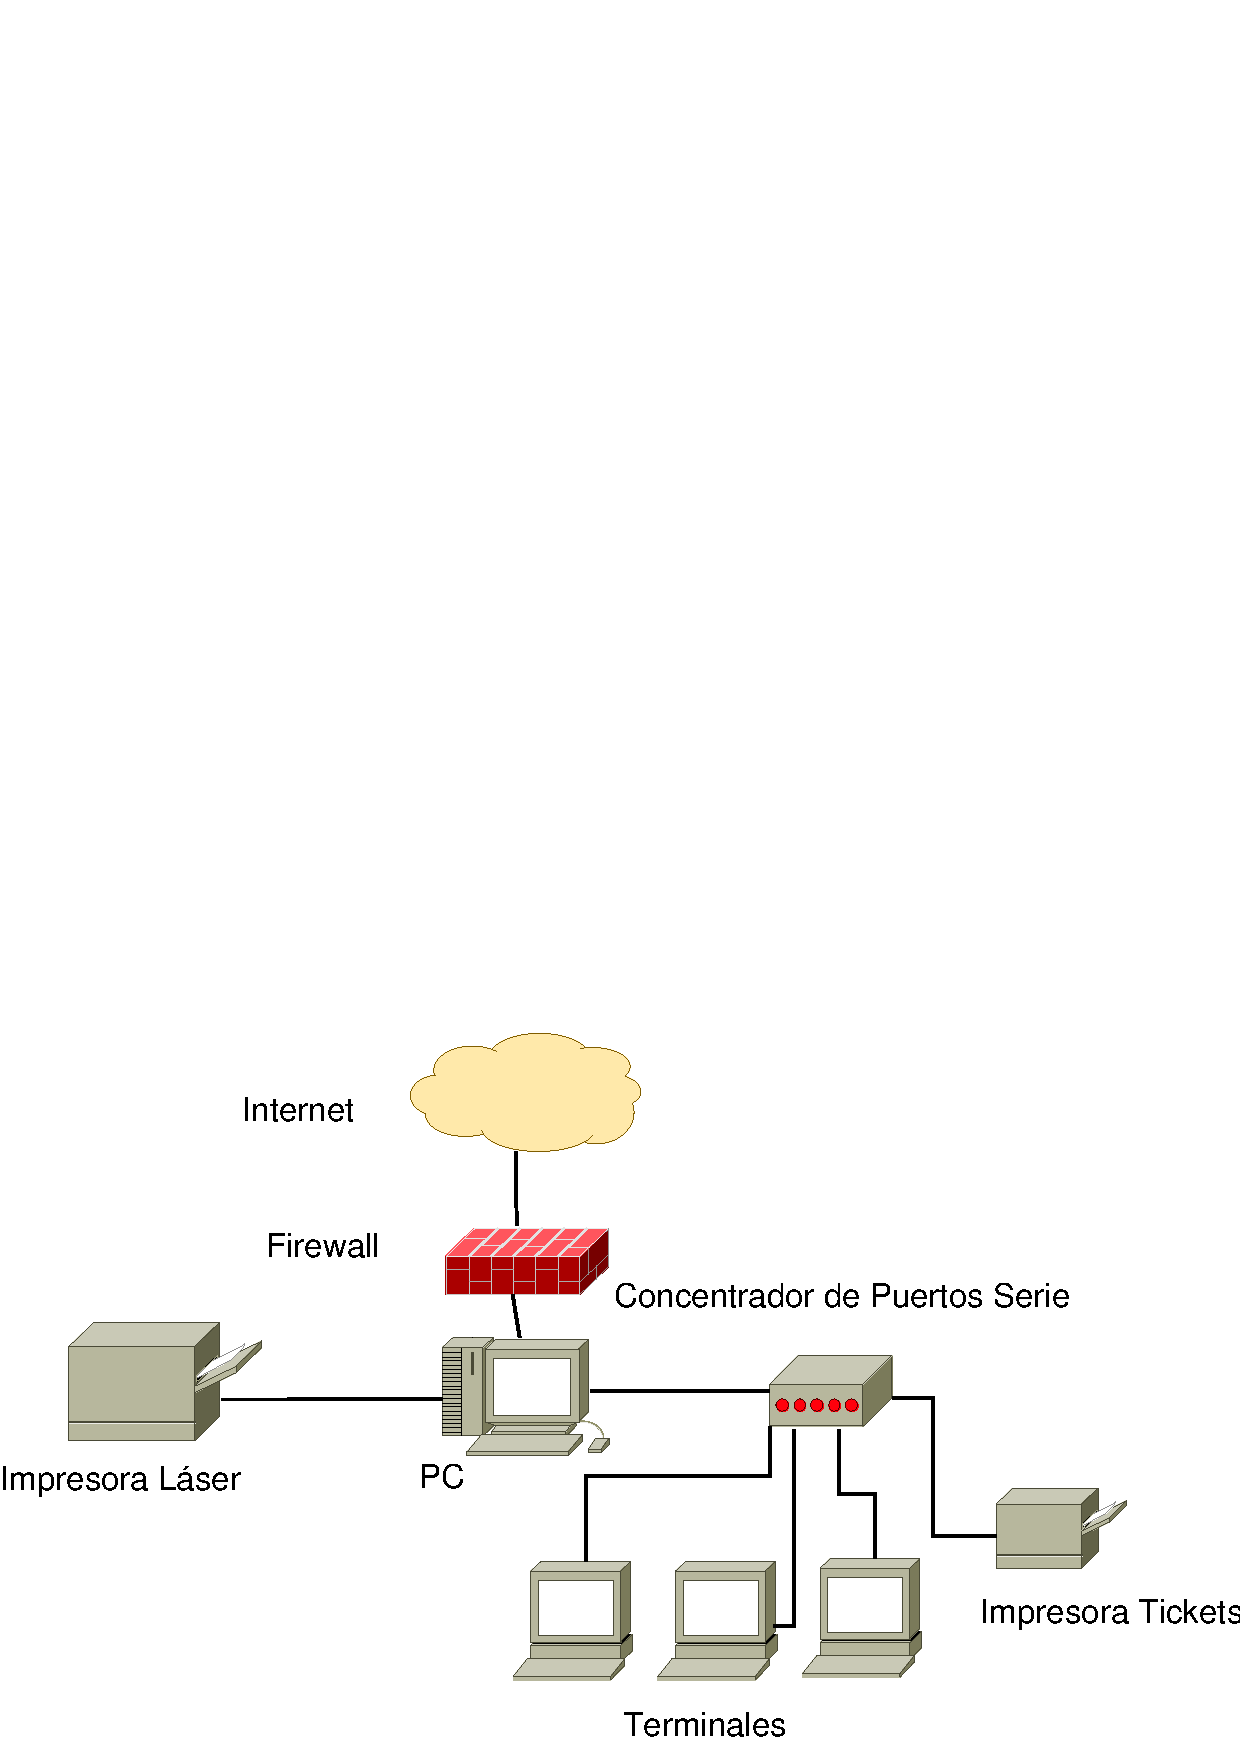
\includegraphics[scale=0.7]{diagrama_ph_sus_1.png}
 \end{center}
 \caption{Sistema en restaurantes PH}
 \label{fig:sist_rest_ph}
\end{figure}

El sistema se compone de una computadora en la cual se ejecuta el sistema punto de venta, se generan reportes propios del punto de venta, el gerente del restaurante consulta el correo electrónico, consulta reportes web propios del restaurante y de la intranet y realiza actividades propias de la operación (como cierres de inventarios, altas/bajas de empleados, etc.). Posee una impresora láser para imprimir documentos, reportes, etc.

La computadora tiene una conexión a internet protegida por un firewall y comunicación a la VPN\footnote{Virtual Private Network, red privada virtual} de la empresa.

Debido a la gran cantidad de equipo que se le puede conectar a la computadora, entre terminales, cajas registradoras e impresoras de tickets, principalmente, se hace uso de un concentrador de puertos seriales, a los cuales se conectan todos los dispositivos. Estos concentradores pueden ser de 6 o 12 puertos y pueden ser conectados más de uno, en caso necesario. La impresora es de matriz y se manda la impresión de los tickets una vez terminada de capturar la orden.

Las terminales, en caso de PH, sirven para tener el punto de venta, que se ejecuta en la computadora, en cada una de ellas, y así poder tomar varias ordenes al mismo tiempo.


La siguiente figura muestra el sistema en KFC a grandes rasgos:

\begin{figure}[htb]
 \begin{center}
  \includegraphics[scale=0.7]{diagrama_kfc_sus_1.png}
 \end{center}
 \caption{Sistema en restaurantes KFC}
 \label{fig:sist_rest_kfc}
\end{figure}

A diferencia del sistema en PH, se cuentan con cajas registradoras en lugar de terminales. Estas cajas registradoras son de la marca Panasonic, y se tienen dos modelos: touchscreen (Panasonic 790, que cuenta con sistema operativo Windows XP Embedded) para restaurantes con un gran número de transacciones y de teclado (Panasonic 5500, usando su propio firmware) para las demás. Se cuenta con un programa desarrollado en la empresa que convierte la salida de las cajas registradoras en registros de venta que son ingresados al punto de venta. Cada caja resgistradora cuenta con su propia impresora de tickets. Dentro del grupo de cajas registradoras se debe tener una especial llamada \textit{master}, la cual es la encargada de trasmitir programación a las secundarias, así como también de recibir información de venta de las demás cajas para ser impresas en el impresor de auditoría. A partir de un desarrollo realizado por mi, esta auditoría se dejó de imprimir y ahora es almacenada de manera electrónica.

\begin{figure}[htb]
 \begin{center}
  \includegraphics[scale=0.7]{panasonic_790.png}
 \end{center}
 \caption{Caja Panasonic 790}
 \label{fig:pana_790}
\end{figure}

\begin{figure}[htb]
 \begin{center}
  \includegraphics[scale=0.7]{panasonic_5500.png}
 \end{center}
 \caption{Caja Panasonic 5500}
 \label{fig:pana_5500}
\end{figure}


